% Appendix Template

\chapter{Technical drawings} % Main appendix title

\label{AppendixD} 

\begin{figure}
	\centering
	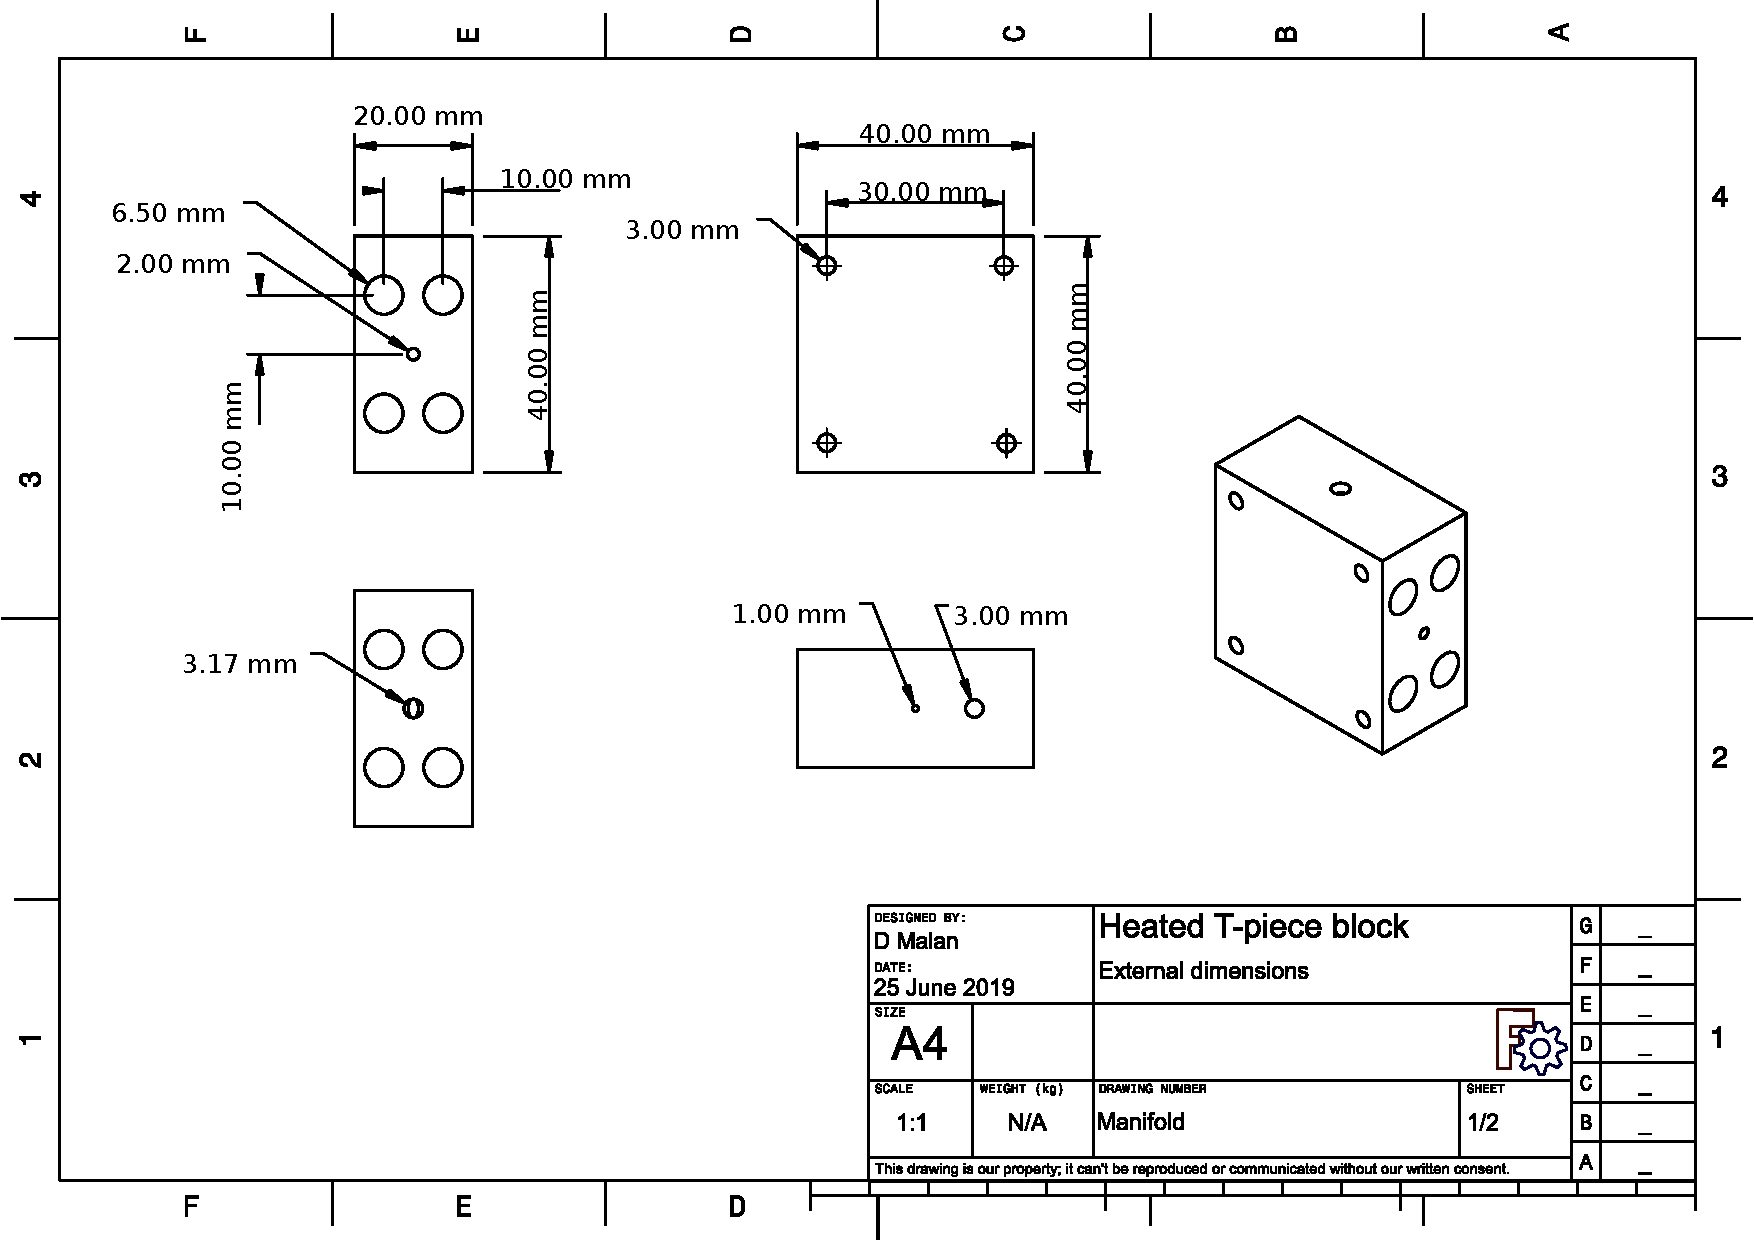
\includegraphics[angle=90, origin=c, scale=0.75]{Figures/ManifoldDimensions.pdf}
	\decoRule
	\caption[Manifold dimensions.]{A technical drawing showing the dimensions of the heated T-piece blocks.}	
	\label{fig:ManifoldDims}
\end{figure}

\begin{figure}
	\centering
	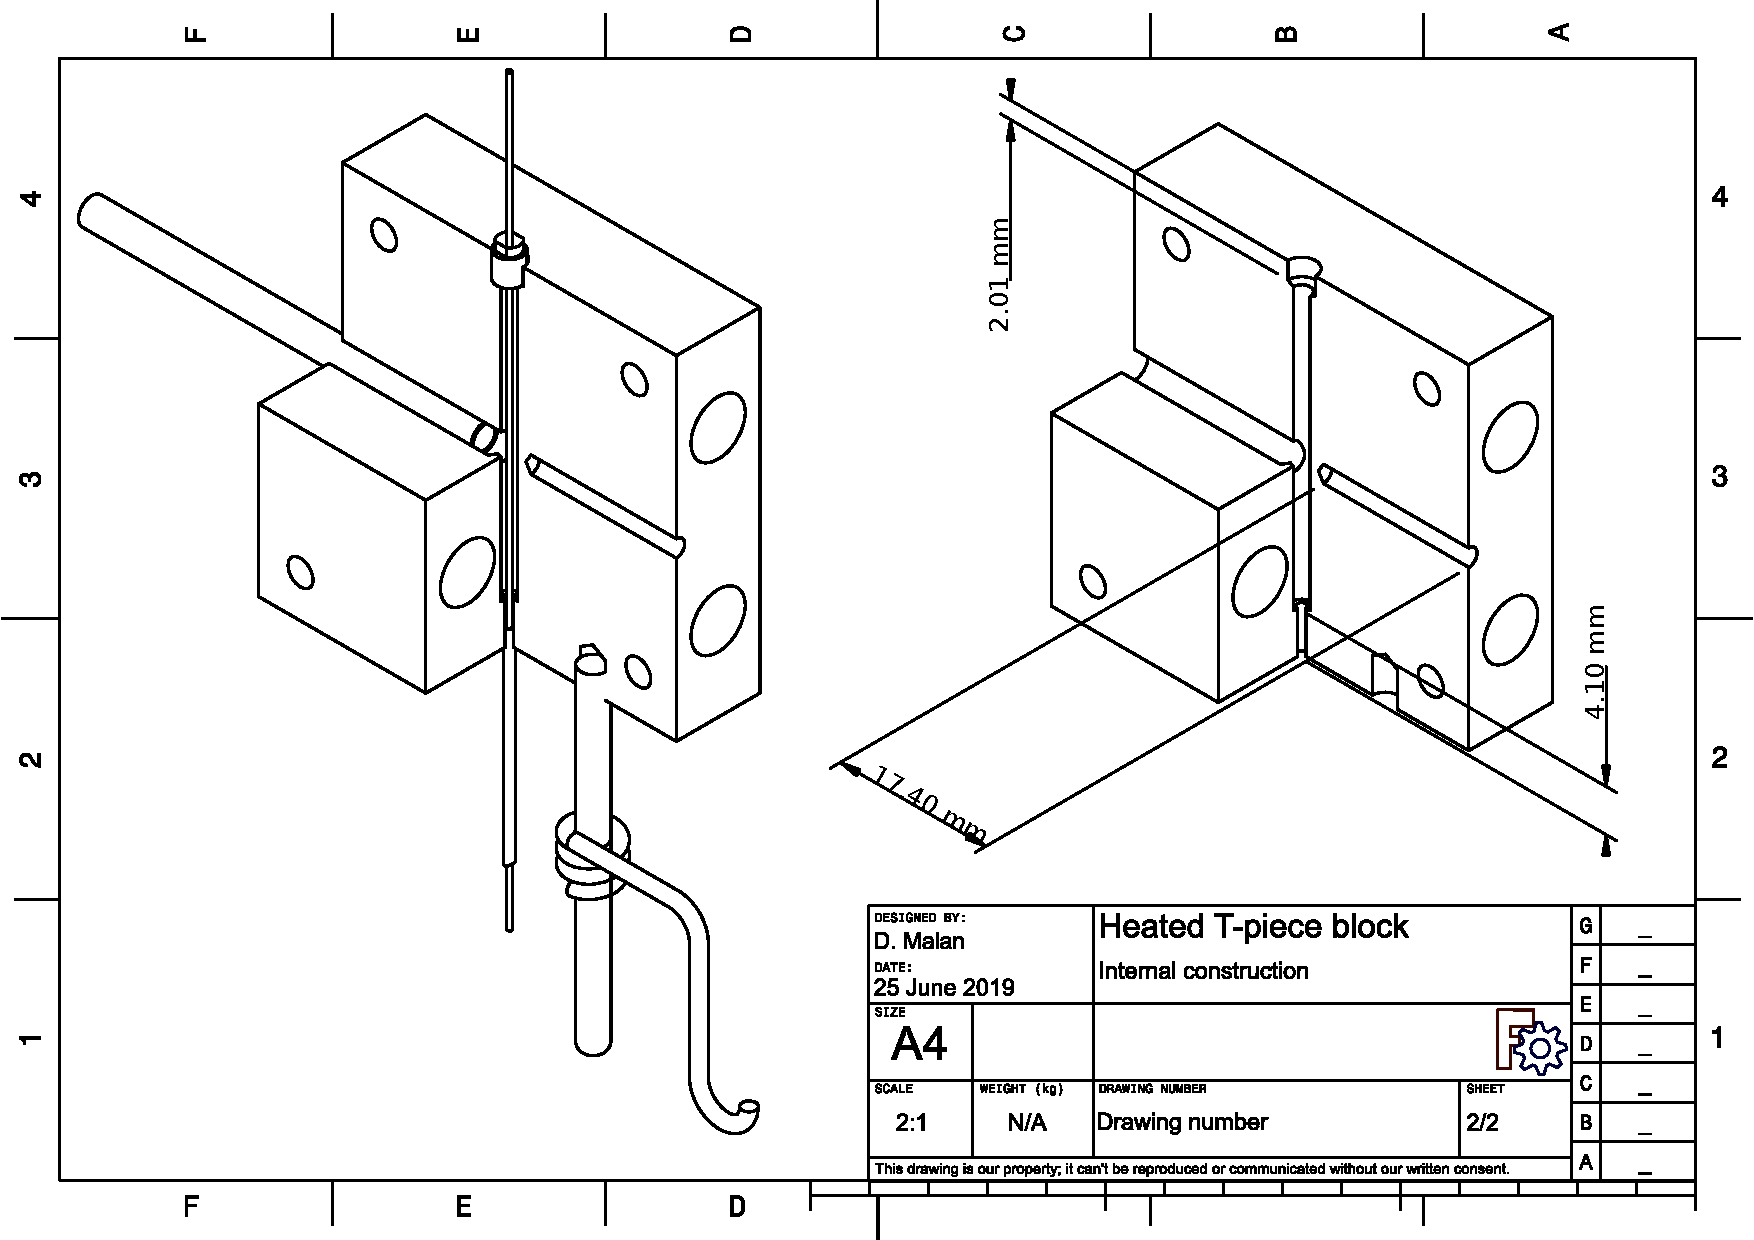
\includegraphics[angle=90, origin=c, , scale=0.75]{Figures/ManifoldAssemby.pdf}
	\decoRule	
	\caption[Manifold assembly.]{A technical drawing of the internal construction and assembly of the heated T-piece blocks.}
	\label{fig:ManifoldAssy}
\end{figure}

\begin{figure}
	\centering
	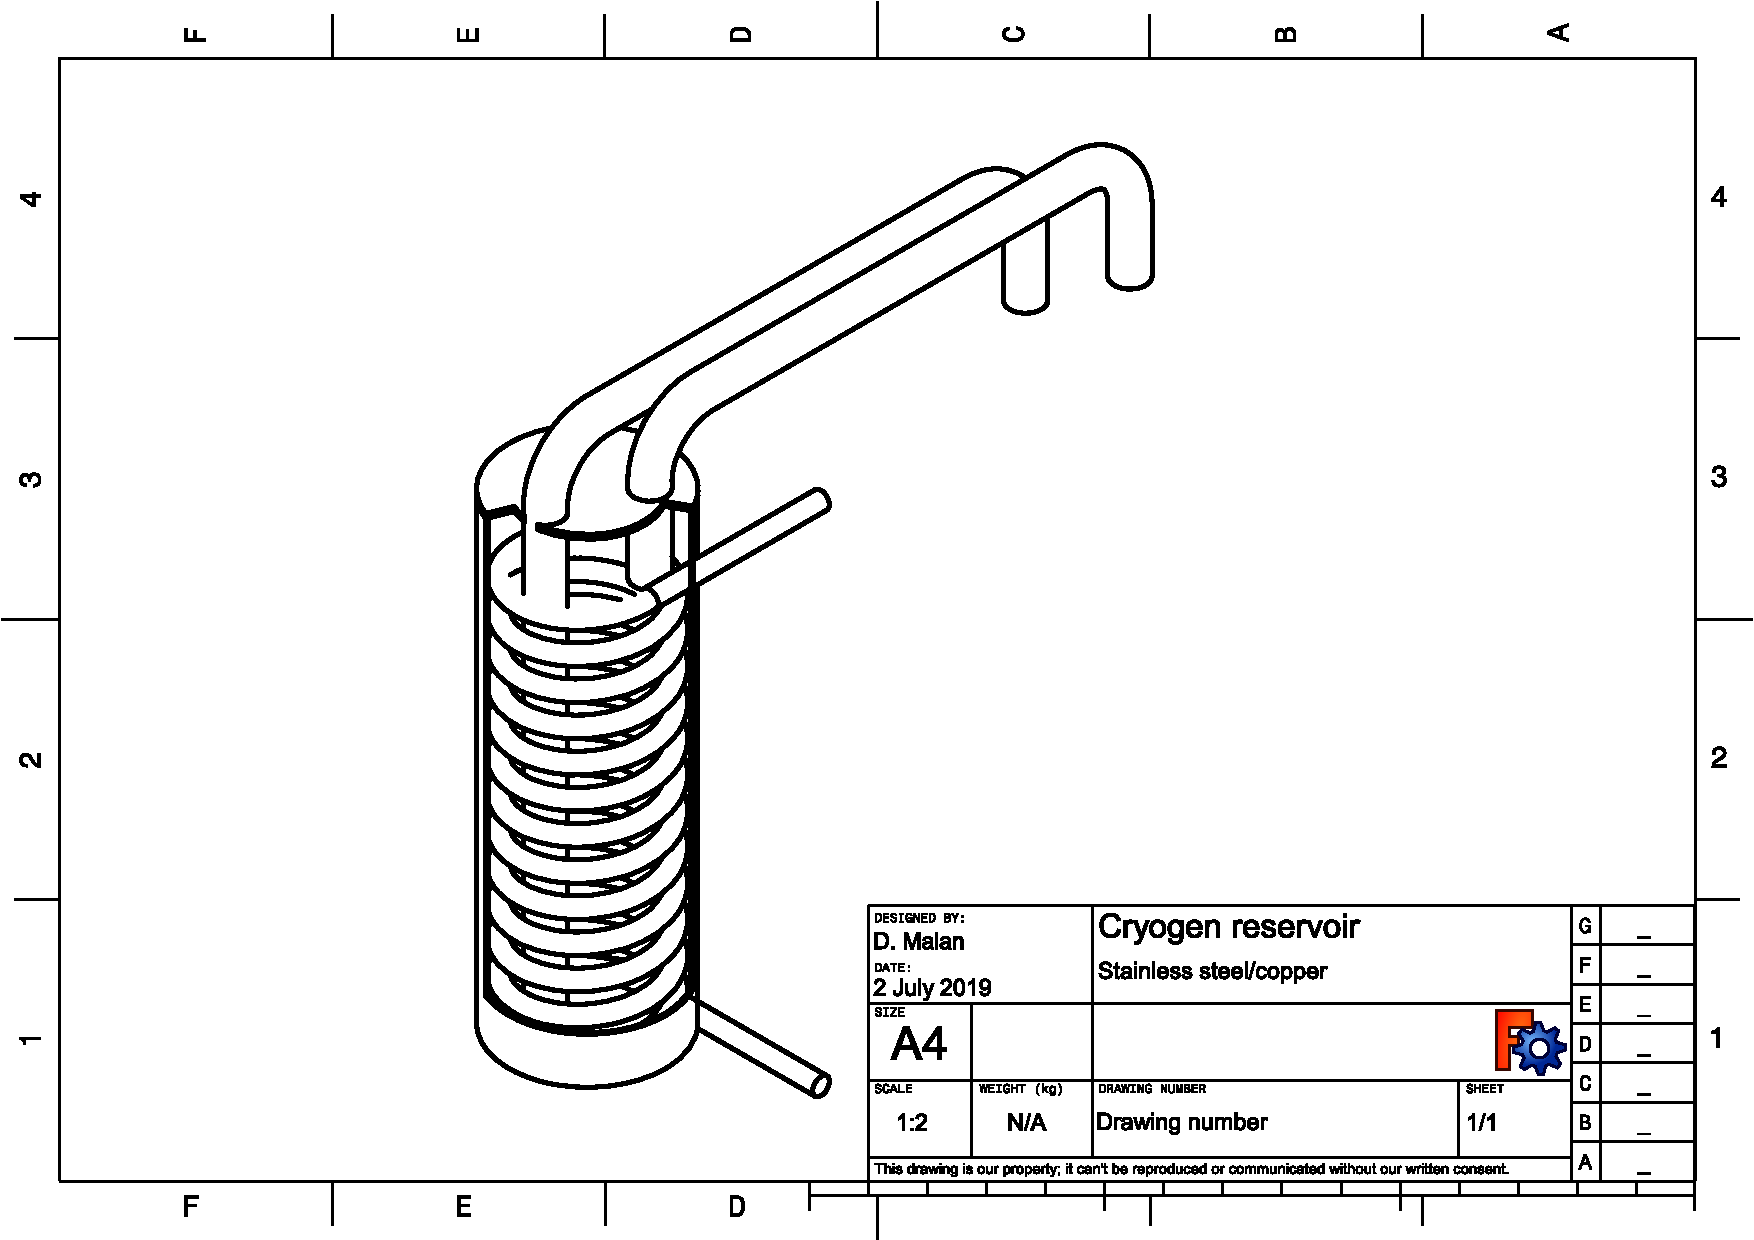
\includegraphics[angle=90, origin=c, scale=0.75]{Figures/CryogenReservoir.pdf}
	\decoRule
	\caption[Coolant reservoir]{Cut-away technical drawing of coolant reservoir.}	
	\label{fig:CryogenReservoir}
\end{figure}

\begin{figure}
	\centering
	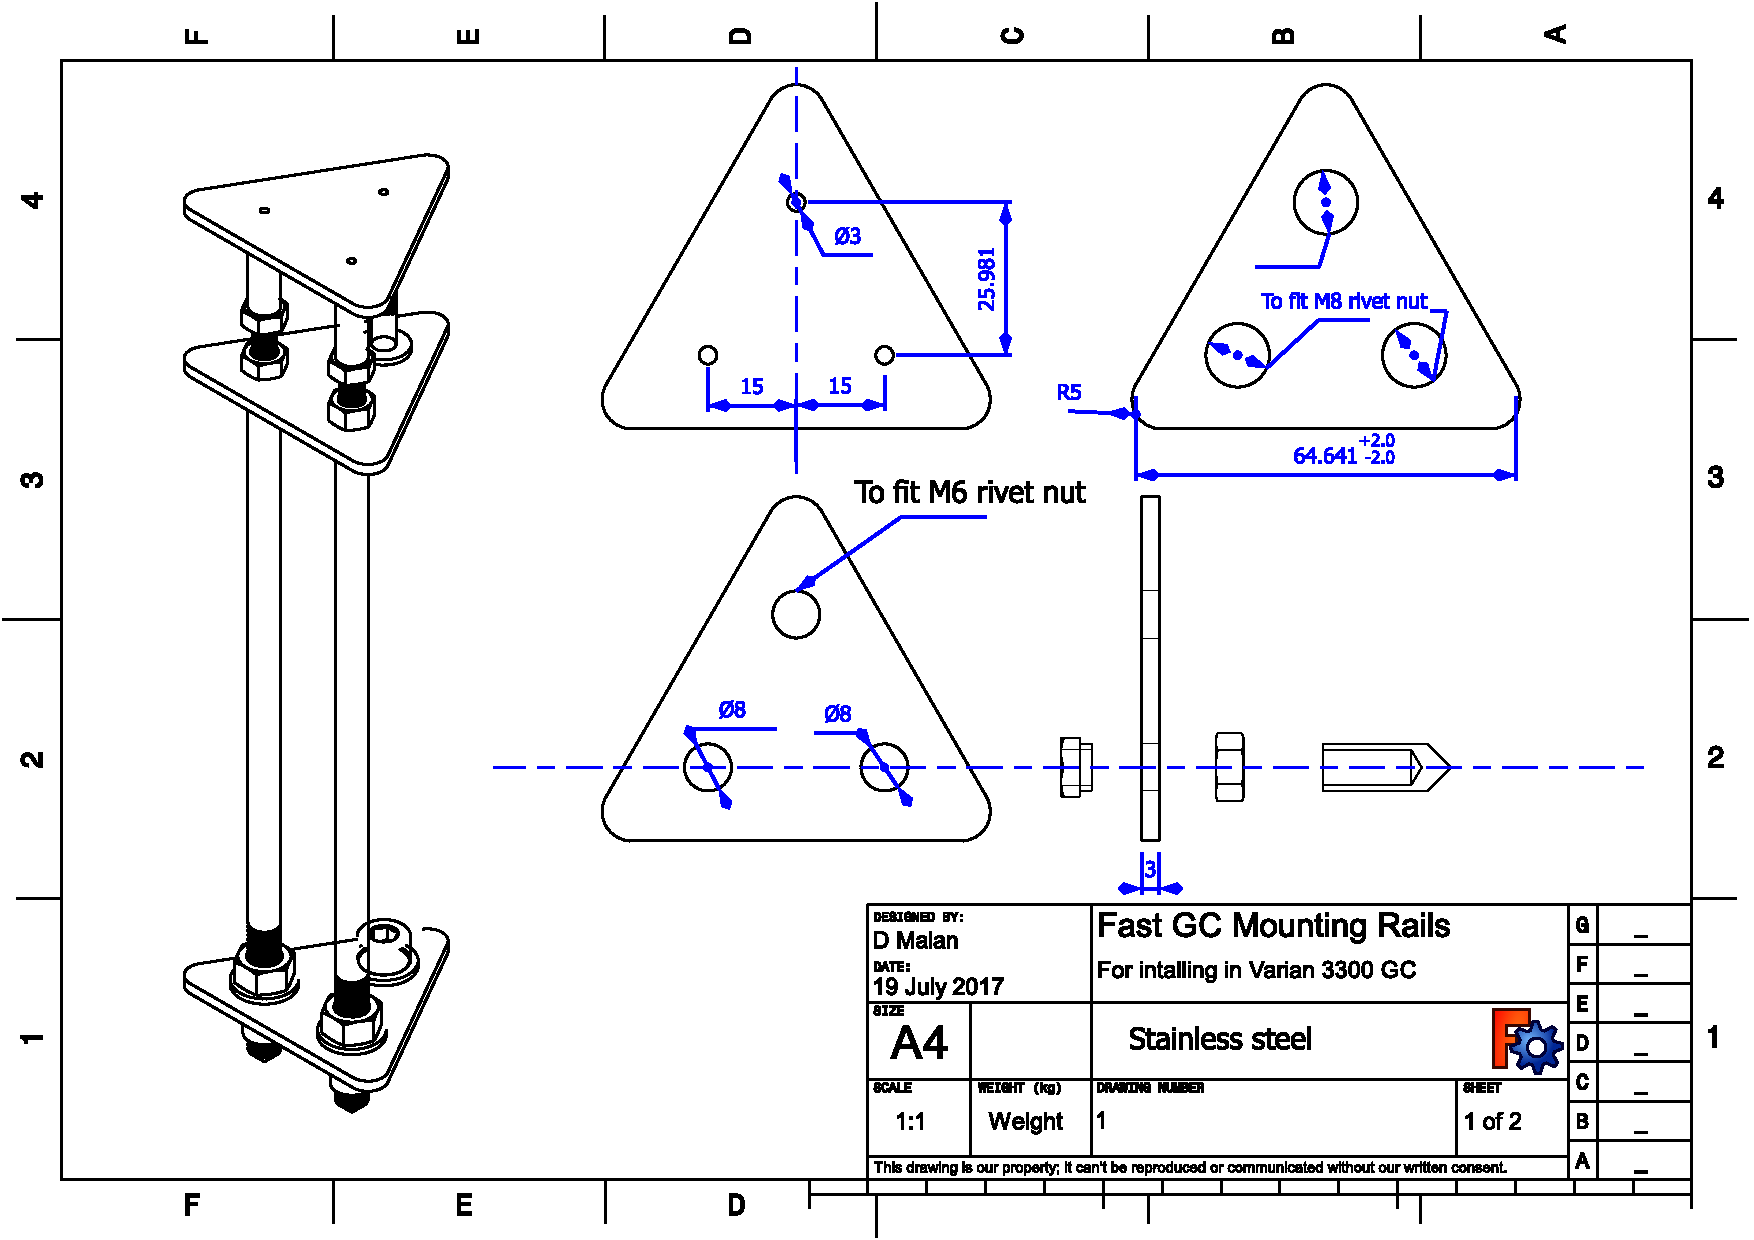
\includegraphics[angle=90, origin=c, scale=0.75]{Figures/RailsDrawing.pdf}
	\decoRule	
	
	\caption[Technical drawing of coaxial heater mounting
	rails]{\label{fig:RailsDrawing}A technical drawing of the rails carrying the
	T-piece mounting block.}
	
\end{figure}

\begin{figure}
	\centering
	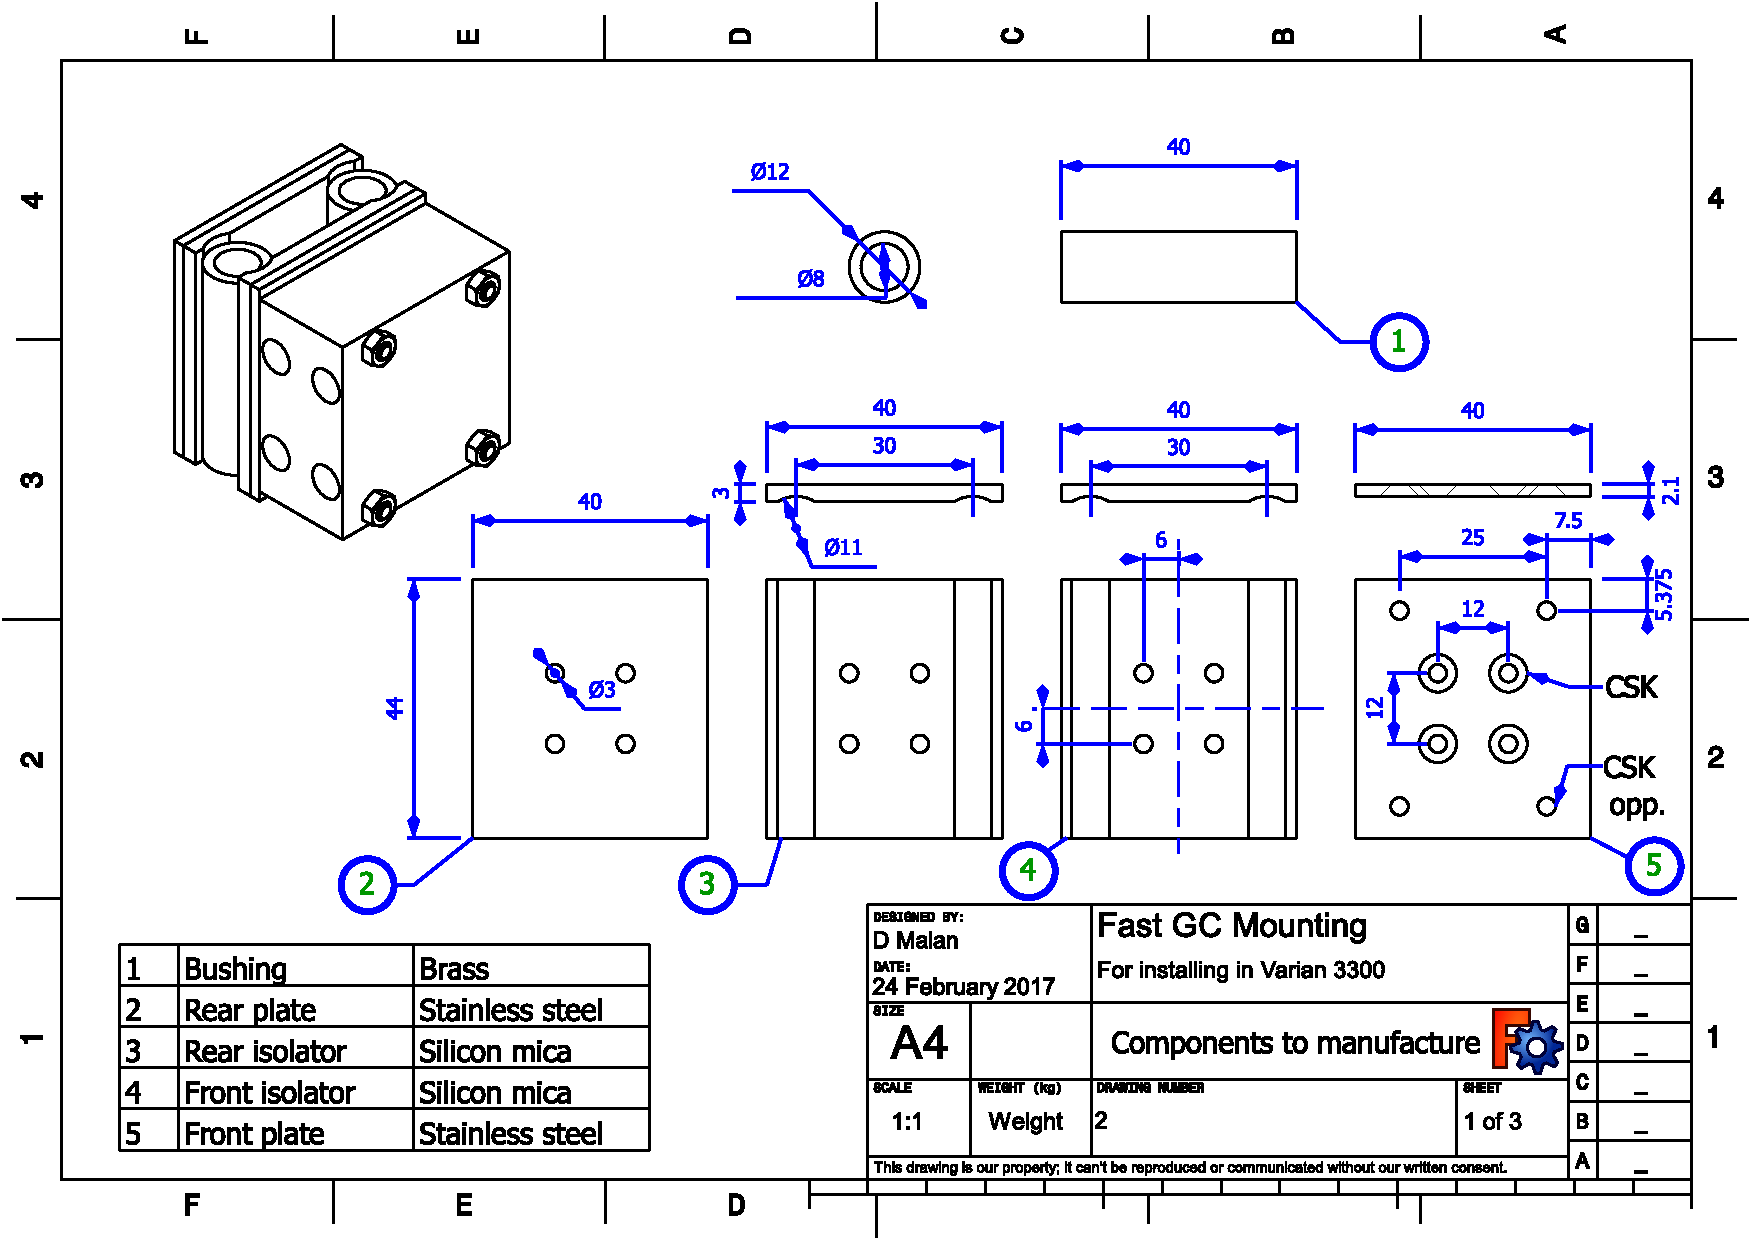
\includegraphics[angle=90, origin=c, scale=0.75]{Figures/CarDrawing1.pdf}
	\decoRule	
	
	\caption[Technical drawing of coaxial heater mounting.]{A technical drawing of
	the T-piece block mounting, showing parts and dimensions.}
	
	\label{fig:CarsDrawing1}
\end{figure}

\begin{figure}
	\ContinuedFloat
	\centering
	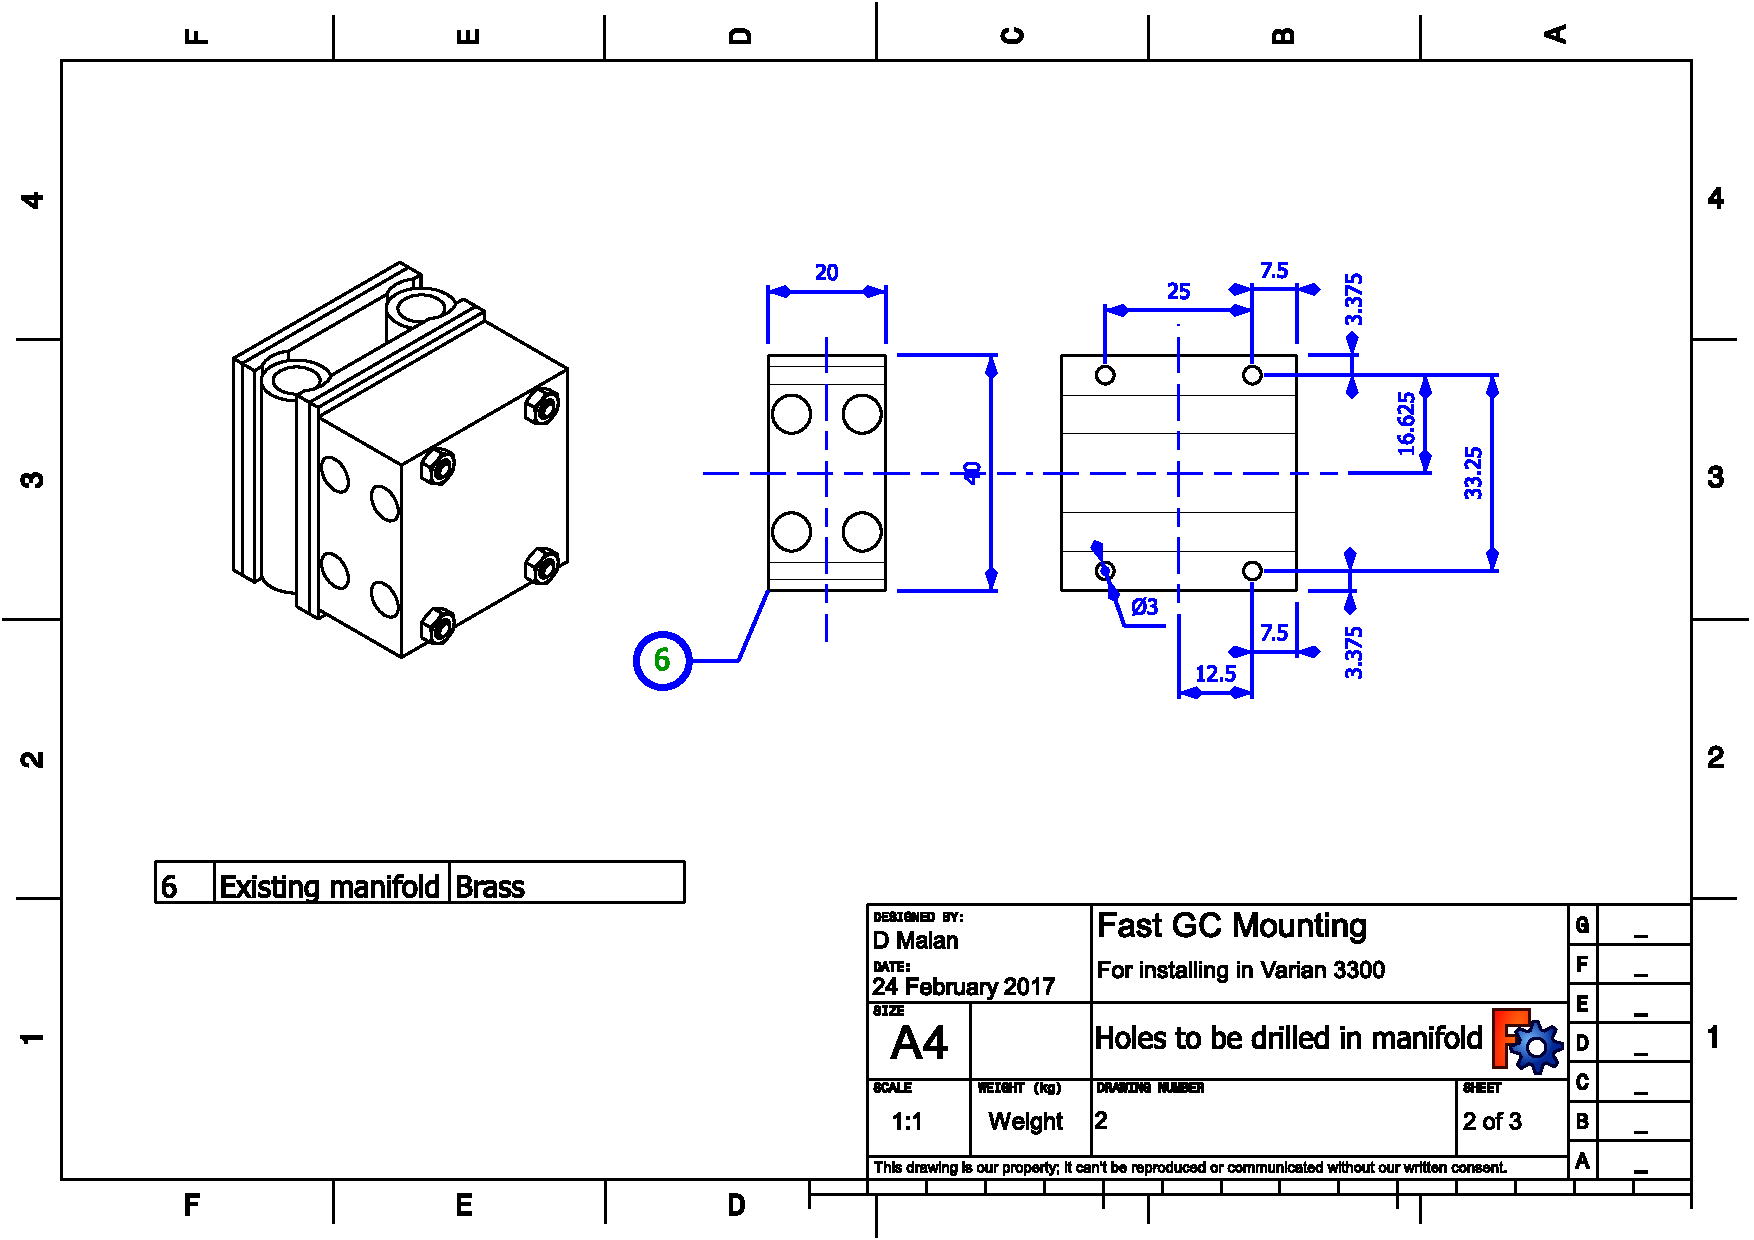
\includegraphics[angle=90, origin=c, scale=0.75]{Figures/CarDrawing2.pdf}
	\decoRule	
	
	\caption[]{(continued) A technical drawing of the T-piece block mounting,
	showing final assembly and dimensions.}
	
	% No label necessary when referred to as part of \ContinuedFloat 
	% \label{fig:CarsDrawing2} 
\end{figure}

\begin{figure}
	\ContinuedFloat
	\centering
	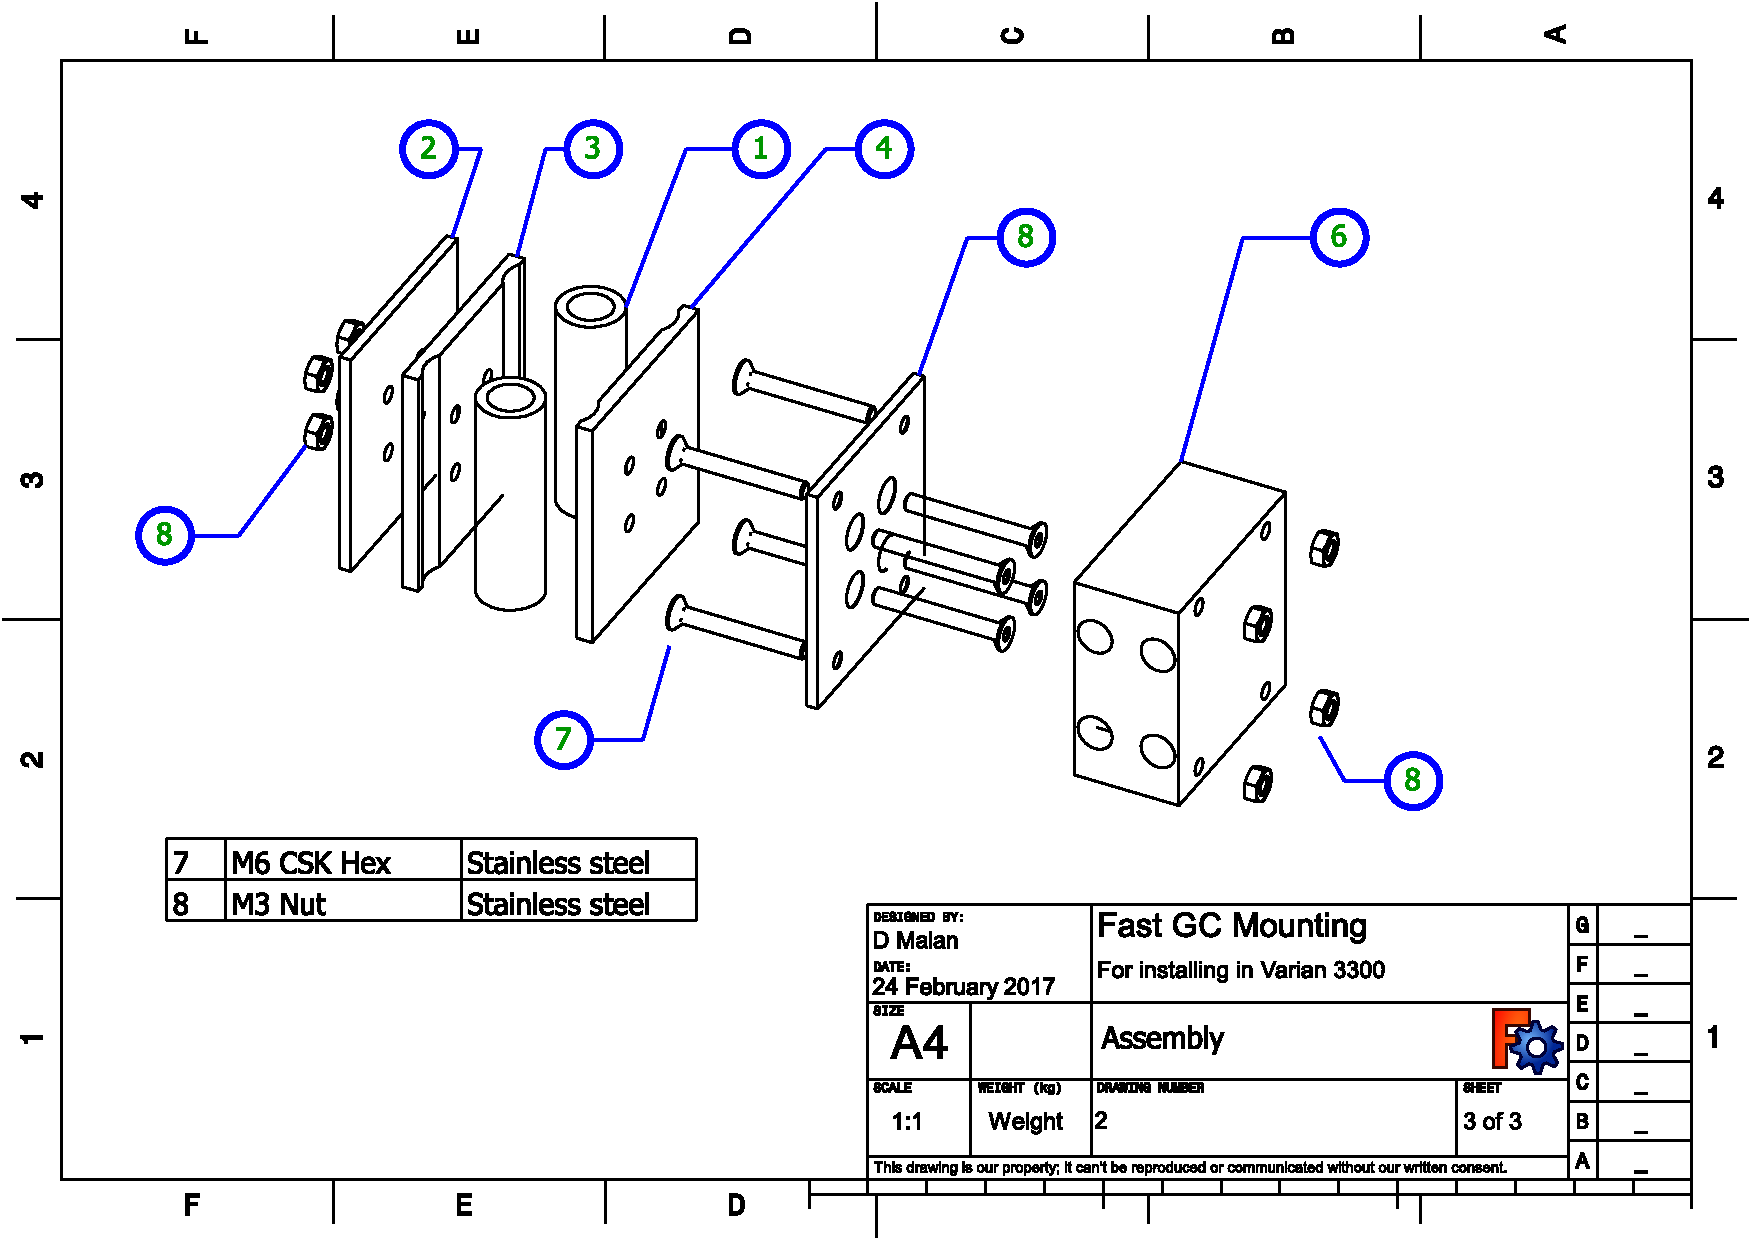
\includegraphics[angle=90, origin=c, scale=0.75]{Figures/CarDrawing3.pdf}
	\decoRule	
	
	\caption[]{(continued) A technical drawing of the T-piece block mounting, showing assembly method.} 
	
	% No label necessary when referred to as part of \ContinuedFloat
	% \label{fig:CarsDrawing3}
\end{figure}


